% Project report for Computational Genomics s2017
% By Han Den (Andrew Id: hdeng1) and Luyi Ma (Andrew Id: luyim)
% Topic : Classification of miRNA using deep-learning method

\documentclass[letterpaper, 11pt]{article}
\usepackage[left=1in, right=1in, top=1in, bottom=1in]{geometry}
\usepackage{multicol}
\setlength{\columnsep}{1cm}
\usepackage{color}
\usepackage{graphicx}
\graphicspath{ {/Project_Report} } 
\newenvironment{Figure}
  {\par\medskip\noindent\minipage{\linewidth}}
  {\endminipage\par\medskip}
\usepackage{caption}
\usepackage{lipsum}
\usepackage{array}


\begin{document}

% title
\begin{center}
{\Large
	\textsc{\textbf Classification of microRNA using Deep Learning Method}
}

\vspace{0.3cm}

\normalsize Project report of Computational Genomics Spring 2017

\vspace{0.5cm}

{\small
	Han Den (Andrew Id: hdeng1)
	
	Luyi Ma (Andrew Id: luyim)
}
\end{center}

% abstract
\begin{abstract}
In recent years, deep learning methods, as a branch of machine learning, have become a powerful tool in many scientific fields. One of deep learning methods, convolutional neural network (CNN), which has an ability of extracting features of high-level abstraction from a minimum preprocessing data, is the most widely used method for classification. In this project, we choose CNN to do microRNA classification and distinguish microRNA from non-microRNA. We use one-hot vectorization model to convert our input sequence into numeric matrices and use these matrices as input to CNN. At last, we train as test our model using miRNA sequences from open-source database and the result shows that our model is efficient in doing miRNA classification.

\vspace{2mm}
\noindent\bfseries{Keywords: miRNA, Convolution Neural Network, Classification, one-hot vectorization}
\end{abstract}

\begin{multicols*}{2}
% introduction
\section{Introduction}
{
MicroRNA (abbreviated miRNA) is a small non-coding RNA molecule (containing about 22 nucleotides) found in plants, animals and some viruses, that functions in RNA silencing and post-transcriptional regulation of gene expression. While the majority of miRNAs are located within the cell, some miRNAs, commonly known as circulating miRNAs or extracellular miRNAs, have also been found in the extracellular environment, including various biological fluids and cell culture media. So it's of great value to distinguish miRNAs from the whole genome and make accurate classifications.
~\cite{miRNA}

In machine learning, a convolutional neural network (CNN, or ConvNet) is a type of feed-forward artificial neural network in which the connectivity pattern between its neurons is inspired by the organization of the animal visual cortex. Individual cortical neurons respond to stimuli in a restricted region of space known as the receptive field. The receptive fields of different neurons partially overlap such that they tile the visual field. The response of an individual neuron to stimuli within its receptive field can be approximated mathematically by a convolution operation. Convolutional networks were inspired by biological processes and are variations of multilayer perceptrons designed to use minimal amounts of preprocessing. They have wide applications in image and video recognition, recommender systems and natural language processing.
~\cite{Convolutional-deep-belief}
~\cite{CNN}
\begin{Figure}
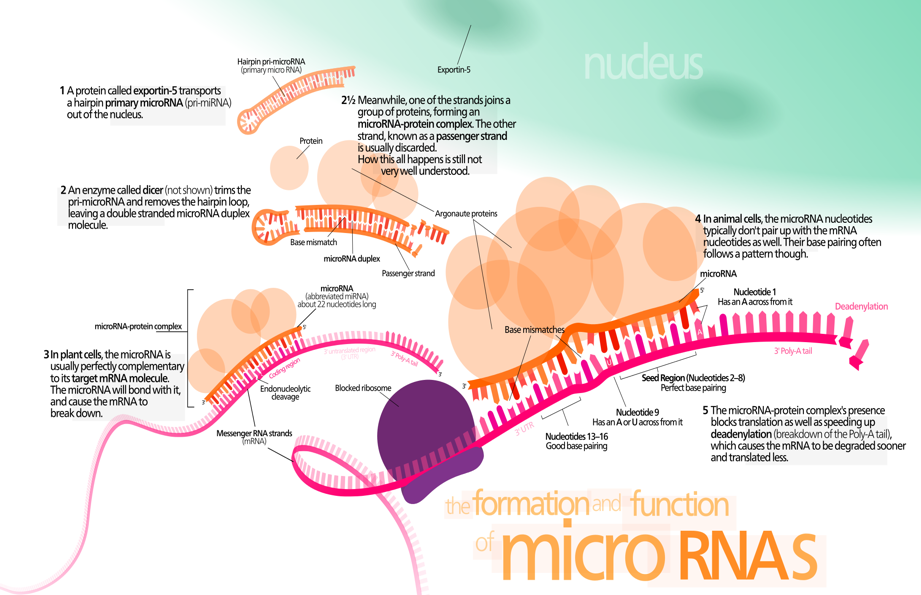
\includegraphics[height = 3.5cm, width = 7cm]{miRNA.png}
\captionof{figure}{\footnotesize Formation and Function of microRNAs: generally, a miRNA molecule has two precursor molecules, pri-microRNA and pre-microRNA. In our model, we use mature miRNA sequences instead of these two precursor sequences. Sequence patterns (seed regions, mismatching regions) could be extracted for miRNA indentification.}
\end{Figure}

The data we use to train and test our model is from miRBase.
~\cite{mirBase} 
MiRBase is the central online repository of miRNA nomenclature, sequence data, annotation and target pre- diction, which first appeared in Oct. 2002 Release 15 contains 14197 miRNA loci from 66 species. From version 5.0, miRBase began to classify miRNAs into different families.
~\cite{miRFam}
We use miRNA sequences from this database as our positive input, meaning that this sequence belongs to the miRNA family.

\begin{Figure}
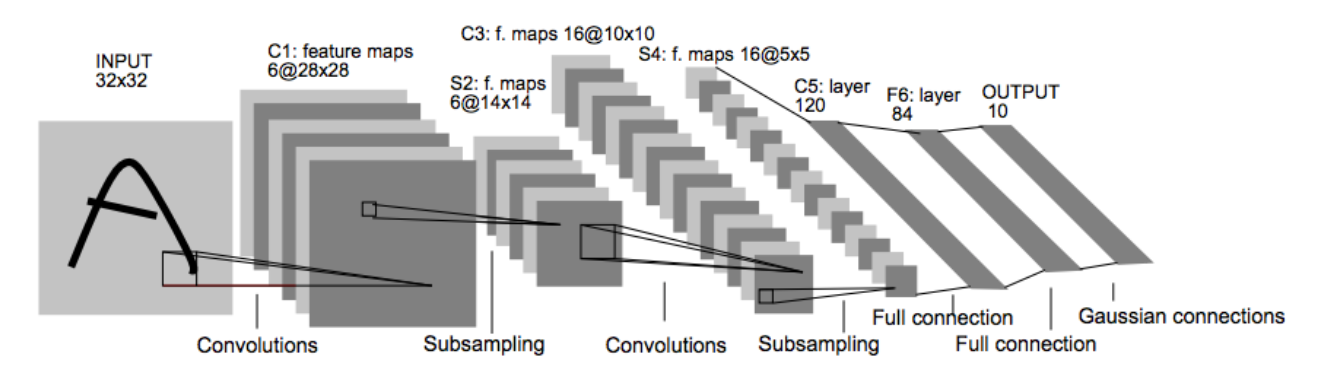
\includegraphics[height = 3cm, width = \textwidth]{lenet.png}
\captionof{figure}{\footnotesize LeNet Structure for Number Recognization: a LeNet contains convolution layers, max pooling layers and some fully-connected layers}
\end{Figure}
}
\section{Methods}
{
\subsection{Word Sequences and Numerical Matrices}
To convert data into vectors, we use a method called one-hot vector. In Fig3 below, we show an example of using one-hot vectors to represent text into the two-dimensional numerical matrix. Assume that we have a small dictionary D which contains 5 words: “I”, “cat”, “dog”, “have”, and “a”. Each word in the dictionary will be represented by a one-hot vector. Then to represent the sentence “I have a dog”, for each region of successive words (in this case is 2 words) we concatenate one-hot vector of each word in the region to generate a vector representing this region. After representing all regions by this mechanism, we will have a 2D numerical matrix representing the sentence.
~\cite{DNA-sequence-classification}
\begin{Figure}
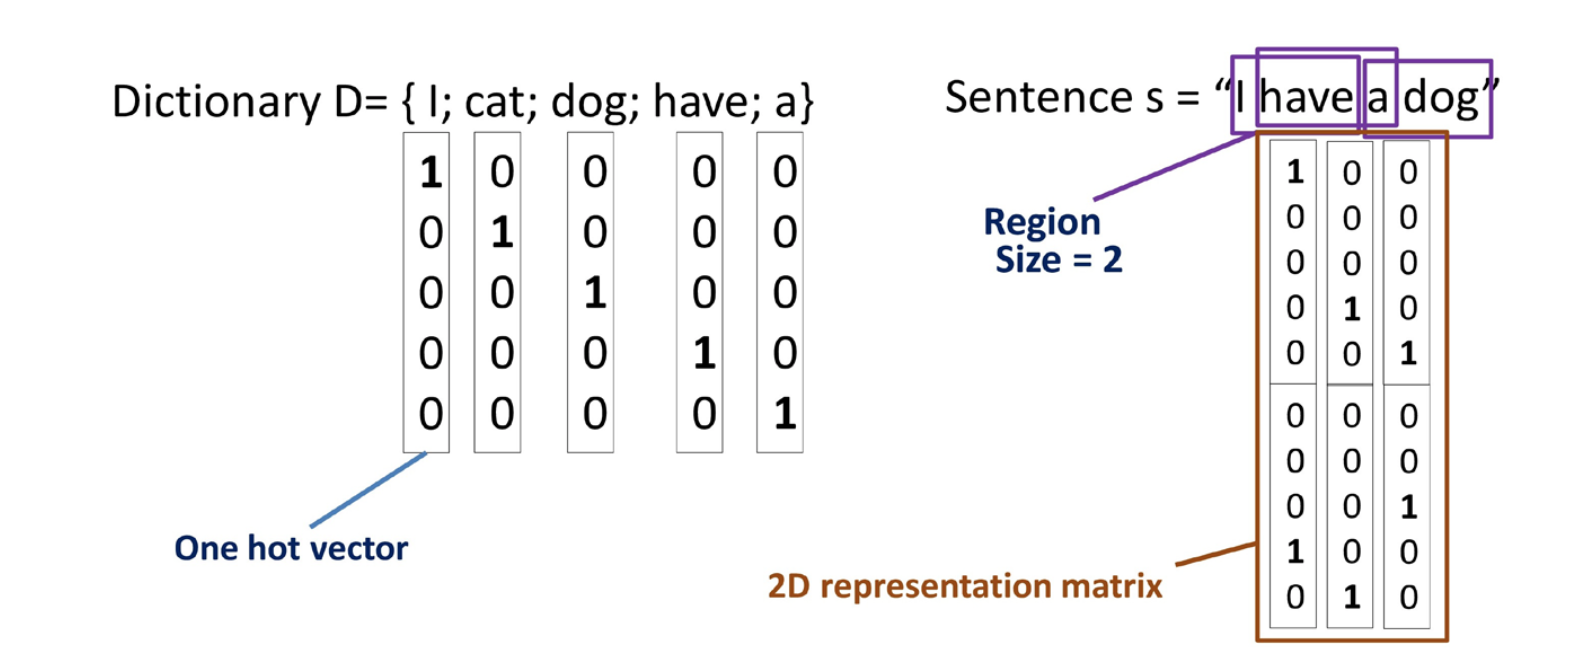
\includegraphics[height = 4cm, width = \textwidth]{word2vec.png}
\captionof{figure}{\footnotesize A simple illustration of one-hot vectorization of a sentence
~\cite{DNA-sequence-classification}}
\end{Figure}

In our experiment, to represent each sequence, we use 3-mers, each can be A, T, C, G, to construct the whole dictionary. So in total our dictionary has 64 different words. And we use the same method with in this picture to convert our sequence into a numerical matrix. The reason why we choose 3-mers is that every 3 nucleotides can be a codon for an amino acid. And the reason why we 	choose concatenate 2 words into a row vector is that we think a word can be influenced by other words, and the one with the greatest influence is the one next to it.

\subsection{Deep Learning Neural Network}
The structure of our CNN is one input layer, one convolution layer, one inner product layer, one ReLU layer, one loss layer. We split data into 10-fold and take 9 fold to train and the rest to test. We use 5 * 5 size of convolution matrix to both consider influence from nearby and avoid noise from distant regions. 
}

\section{Implementation details}
{
\subsection{Data Generation}
\indent Generally, our dataset is generated by mixing sequences with positive labels (miRNA sequence) and sequences with negative labels (non-miRNA sequence). For sequences with positive labels, we download fasta-format file containing sequences of mature miRNA from miRBase[citation miRBase] and extract sequence information for data processing. Because we want to identify potential miRNA sequence on DNA level, we simply parse all miRNA sequences and convert all character 'U' to 'T'. These sequences are our positive data. For negative dataset, we fail to find databases with relevant information and decide to permutation methods to generate random sequences excluding existed positive dataset sequence.

To model the sequence generation process, we first compute the distribution of four nucleotides ('A', 'T', 'C' and 'G') in our positive dataset. Figure 4 shows the distribution of four nucleotides. We notice that four nucleotides have different empirical probabilities to occur in the positive dataset. However, in the whole genome, all these four nucleotides share the same probability to occur in a random sequence. So we uniformly select nucleotides when generating random sequences. 
\begin{Figure}
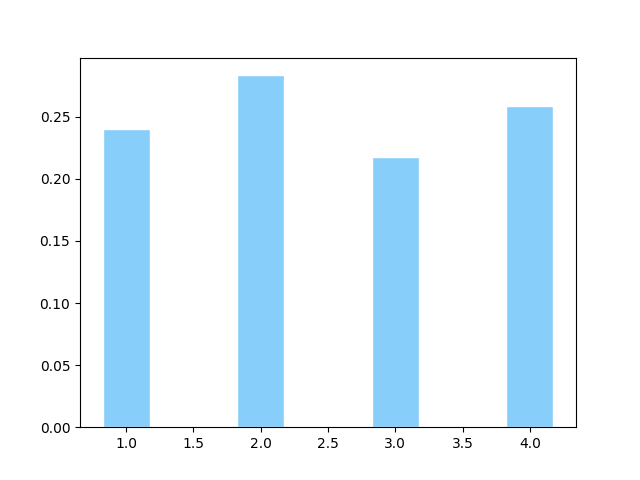
\includegraphics[height=5cm, width=\textwidth]{ATCG.png}
\captionof{figure}{\footnotesize{Distribution of A, T, C and G in positive dataset}}
\end{Figure}
To define the length of random sequences, we also collect the distribution of sequence length in the positive dataset shown in Figure 5. In 35828 records of the positive dataset, we notice that sequences with length ranging from 17 to 27 dominate the dataset. We compute the frequency of sequences with length from 17 to 27 and normalized them by the sum of frequencies of these 11 categories for modeling a categorical distribution of the sequence length.
\begin{Figure}
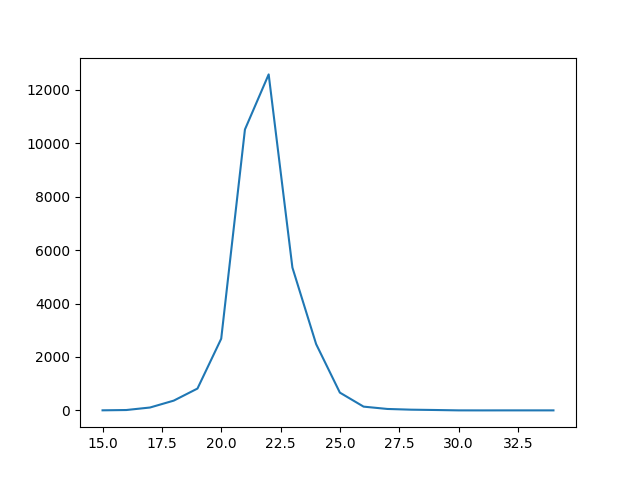
\includegraphics[height=5cm, width=\textwidth]{lendistribute.png}
\captionof{figure}{\footnotesize{Distrubition of sequenc lengths in the positive dataset}}
\end{Figure}
We use these two models to generate random sequence and exclude sequences contain sequences in the positive dataset or are contained by sequences in the positive dataset. For example, for each random sequence, we first use a categorical distribution of sequence lengths to generate a random length of the new sequence and then uniformly sample nucleotides to generate a random sequence with this length. Then, we compare this sequence with all the sequences that have been generated. If there are repeats, we discard this sequence. If there are no repeats, we further compare this sequence with sequences in the positive dataset and only store the sequence that is unique. We generate 35828 sequences based on the protocal mentioned above as our negative dataset.
\subsection{Sequence Vectorization}
We use one-hot vectorization method to vectorize the sequences. There is a prior here that we believe sequences can be parsed and chunked in 3-mer tokens because codons are 3-mers. So there are 64 different 3-mers. We numerate them, sort them in the lexicographical order and produce a lookup table by generating one-hot vector for each 3-mer (shown in Figure 3). We use this lookup table to vectorize sequences.
\begin{Figure}
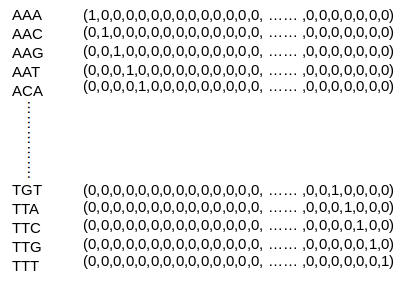
\includegraphics[height=5cm, width=\textwidth]{lookup_table.png}
\captionof{figure}{3-mer vectorization and Lookup table}
\end{Figure} 
\subsection{Input Data Processing}
We parse each sequence by sliding a window with the size of 3 nuleotides and match the vector of this 3-mer. More specifically, we stack vectors of 3-mer vertically and produce an "image" of this sequence. For each row of this "image", we stack vectors of two adjacent 3-mers horizontally. Finally, we have a matrix representing the sequence "image" with $|length|-3$ rows and 128 columns. Based on the sequence length distribution, we choose 22 as our optimal sequence length, trimming sequences with a length greater than 22 to 22 nucleotides and padding zeros to the vectors. We randomly select 3 sequences from the positive dataset and 3 sequences from the negative dataset to visualize their sequence images. We can see that "TGGAATGTAAAGAAGTATGTA" from the positive dataset and "CATTAACCTTCATATTTCCTT" from the negative dataset arewith length of 21 nucleiotide and the 22\textsuperscript{th} rows in both images don't have red squares, which indicates the zero padding in their matrix.
\begin{Figure}
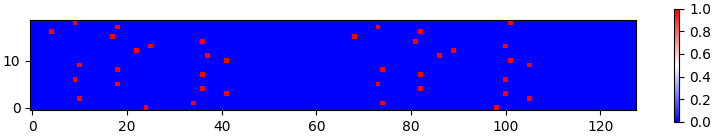
\includegraphics[height=2cm, width=\textwidth]{pos1.png}
\captionof{figure}{Sequence "TGAGGTAGTAGGTTGTATAGTT" vectorization (from the positive dataset)}
\end{Figure} 
\begin{Figure}
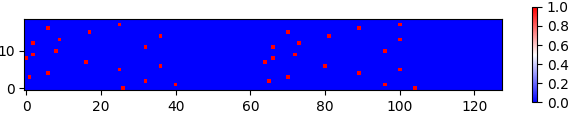
\includegraphics[height=2cm, width=\textwidth]{pos2.png}
\captionof{figure}{Sequence "TGGAATGTAAAGAAGTATGTA" vectorization (from the positive dataset)}
\end{Figure} 
\begin{Figure}
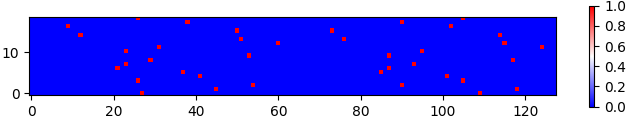
\includegraphics[height=2cm, width=\textwidth]{pos3.png}
\captionof{figure}{Sequence "TGCTGGTTTCTTCCACAGTGGTA" vectorization (from the positive dataset)}
\end{Figure} 
\begin{Figure}
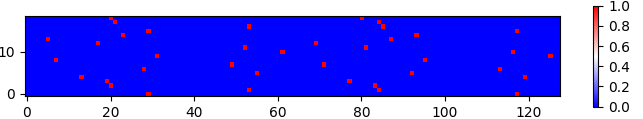
\includegraphics[height=2cm, width=\textwidth]{neg1.png}
\captionof{figure}{Sequence "TCTTACTCATCCTATTCTTTAA" vectorization (from the negative dataset)}
\end{Figure} 
\begin{Figure}
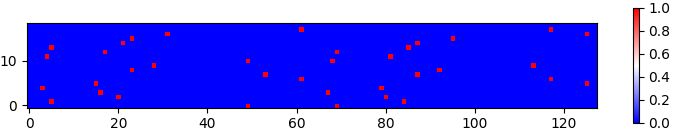
\includegraphics[height=2cm, width=\textwidth]{neg2.png}
\captionof{figure}{Sequence "CATTAACCTTCATATTTCCTT" vectorization (from the negative dataset)}
\end{Figure} 
\begin{Figure}
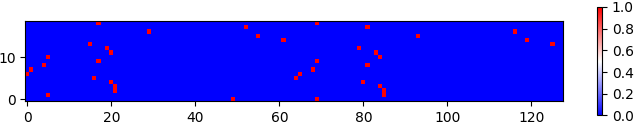
\includegraphics[height=2cm, width=\textwidth]{neg3.png}
\captionof{figure}{Sequence "CATTTTAAATATTACCTCTATT" vectorization (from the negative dataset)}
\end{Figure} 
\subsection{Convolution Neural Networks}
We use LeNet as our basic convolution neural network structure and implement it with some changes that fit our input data. For neural network implementation, we use backpropagaion to compute the loss function of the whole network and use mini-batch stochastic gradient descent to optimize loss function. The overall structure of our neural network is listed in Table 1.
\begin{center}
\begin{tabular}{ || m{2cm} | m{5cm} ||}
\hline
\textbf{Layers} & \textbf{Configure} \\ 
\hline
Input & size: 19 x 128 x 1 (one channel) \\
\hline
Convolution & $k$ (window size) = 5, $s$ (stride) = 1, $p$ (padding size) = 0, $n$ (number of filters) = 20 \\
\hline
Inner Product & $n$ = 500 \\
\hline
ReLU & $n$ = 2\\
\hline
SoftMax  &  $n$ = 2\\
\hline 
Loss & Negative Log-Likelihood\\
\hline
\end{tabular}
\vspace{2mm}

\footnotesize{Table1. Convolution Neural Network architecture and Configure}
\end{center}

The loss function used here is the negative log-likelihood of the neural network based on the parameters and can be removed after finishin training for prediction.

We mix sequence images of the positive dataset and the negative dataset, shuffle the order of images and choose the first 90\% data as the training set and the rest as the test set. Because of the computation complexity, we just train our model without using cross validation to optimize hyperparameters like the size of convolution matrix and the stride size. For mini-batch stochastic gradient descent, we choose 64 as our batch size. In other words, in each iteration, we use continuous 64 images as the data input from a random start point, compute the gradient of these 64 batch and optimize the loss function. We train our model 1500 iterations. Our program compute all the operations (convolution, pooling and gradient) in a single process.
}

\section{Results and Conclusions}

{
\subsection{Training Record}
We train our model with 1500 iterations and notice that sometimes our model can achieve almost 100\% train accuracy while sometimes only about 50\%. To record this phenomenon, we train our model 2000 iterations many times with random start points and visualize the history of two training processes amount all attempts. Following figures show the record of training process. We think that the loss function of our model is not convex and there are at least two local optimal value, one is responsibel for the training accuracy of $\approx$ 50\% and the other is for the training accuracy of $\geq$ 98\%. For the model with the training accuracy of $\approx$ 50\%, we guess that the model may (1) doesn't learn anything and randomly "guesses" a result, (2) or just randomly learn one of the two sequence patterns (miRNA sequence or non-miRNA sequences). For the reason of limit time, we don't design test case to prove our guess. But it is true that the initiation of training (picking a start point) is very important for our model because the stochastic gradient descent method doesn't guarantee to find the global optimal value for a non-convex function. It can be a work of refining our model and its implementation. 
\begin{Figure}
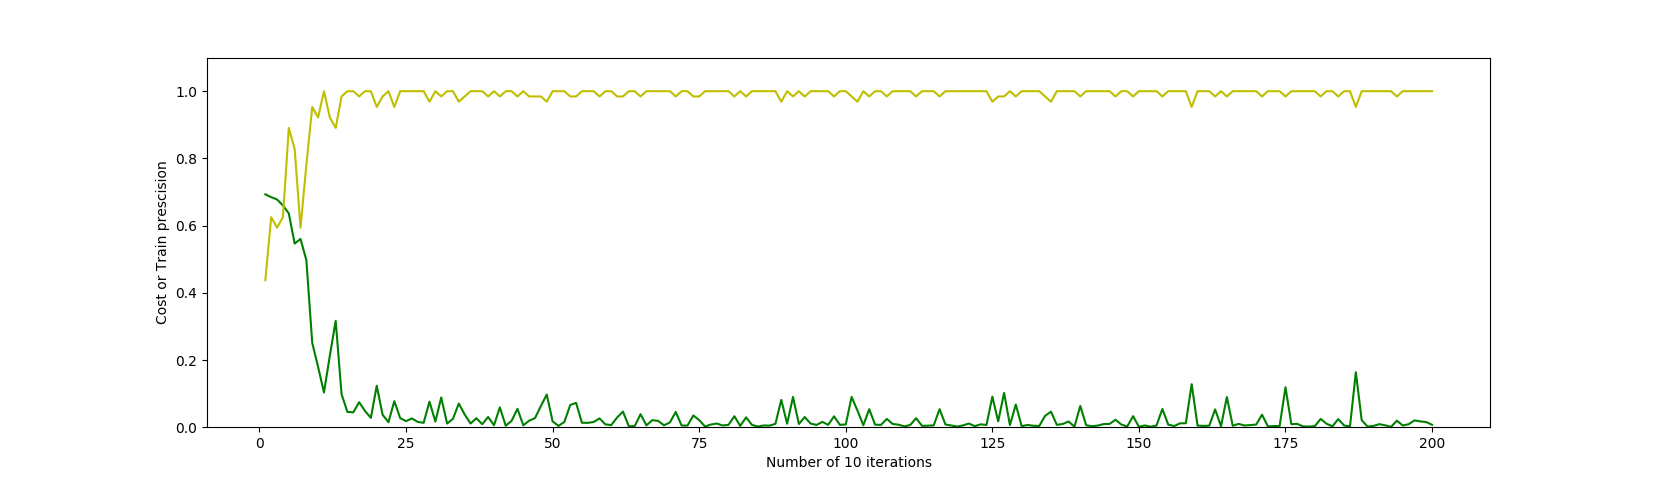
\includegraphics[height = 3cm, width = \textwidth]{correct.png}
%\captionof{figure}{Training Record: The "YellowGreen line" indicates the training accuracy and the"Green line" indicates the cost(value of the loss function).}
\vspace{2mm}
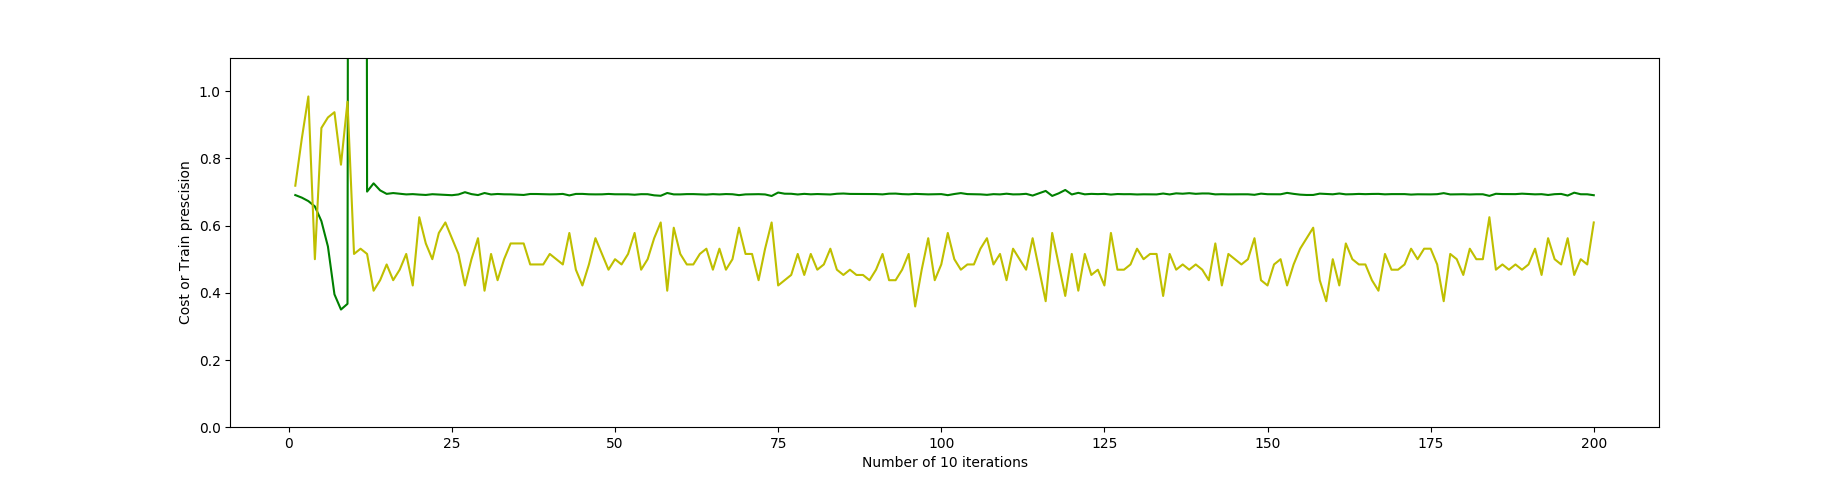
\includegraphics[height = 3cm, width = \textwidth]{incorrect.png}
\captionof{figure}{\footnotesize Training Record: The "YellowGreen line" indicates the training accuracy and the"Green line" indicates the cost(value of the loss function). The upper subfigure shows the record of a model with $\geq$ 98\% training accuracy while the bottom subfigure shows the record of a model with $\approx$ 50\% training accuracy.}
\end{Figure}


\subsection{Performance}
After 1500 iterations, we choose a model with highest average training accuracy and use the parameters of this model to predict the labels of sequences in the test set. To make it generic, our test set is sampled randomly from our whole dataset. We use F-score to evaluate model's performance. Tabel 2 shows the results.
\begin{center}
\begin{tabular}{||m{2cm}|m{5cm}||}
\hline
\textbf{Items} & \textbf{Details or Valuse}\\
\hline
Test set & 7171 sequences with both positive sequences and negative sequences\\
\hline
Accuracy & 0.995259\\
\hline
Average Precision & 0.997593\\
\hline
Recall & 0.990444\\
\hline
F1-score & 0.995199\\
\hline
\end{tabular}
\vspace{2mm}

\footnotesize{Table2. Perfomance of the CNN model}
\end{center}

We compare the test accuracy of another classifier using Logistic Regression. Here is the result shown in Figure 14. We can see that the convolution neural network has a test accuracy more than 99\% while the Logistic Regression has a test accuracy less than 90\%. Our model has better performance on this classfication task than the Logistic Regression model.
\begin{Figure}
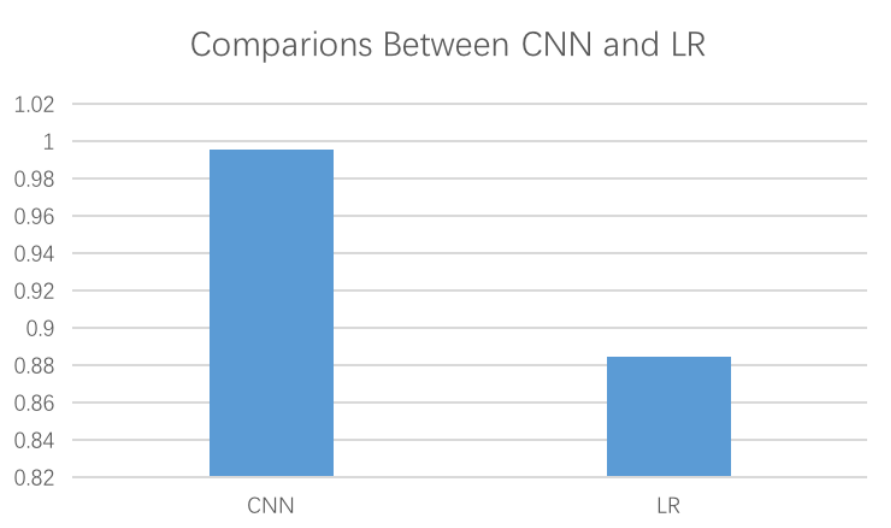
\includegraphics[height = 4cm, width = \textwidth]{com.png}
\captionof{figure}{\footnotesize Test accuracy: Convolution Neural Network (CNN) and Logistic Regression (LR)}
\end{Figure}
\subsection{Discussion and Conclusions}
Our model achieve very high F1-score on this classification task. However, it is more complicated than other classifier like Logistic Regression and SVM. So there is a trade-off between the accuracy and computation complexity. Also, our classification task is relative simple compared with a real-world classification task -- identifying the subtype of a miRNA sequence. Currently, we finish the step of recognizing a chunk of DNA sequence that is a potential pot encoding miRNA sequence. Based on this step, we can approach many interesting discoveries in transcriptome. By processing the whole genome sequence data, our model may filter out canditate DNA sequence segments that are responsible for encoding miRNA, which is a genome-wise miRNA-mining. We can adjust our model to a new convolution neural network with different convolution filters that parse and extract information of substructure of a miRNA molecule.

Our model still has some drawbacks. The first one is model complexity. For this relatively simple classification task, our model need more memory and time to finish training and prediction. One solution for this problem is to adjust our program to be multi-process. Another improvement could be using GPUs. The second drawback is that the output of our model is relatively simple, just a binary classification. To extend the application of our model, in addition to adding new convolution filters, we can adapt other classifiers in our neural network. For example, we can use CNN to extract information from sequence image, and use a decision tree to classify an input into more subtle classes.
}

\section{Code}
We upload our code and other project details to our public Github https://github.com/
ComputationalGenomics-Project/CNN-for-miRNA-classification.
\end{multicols*}

\newpage
\begin{multicols*}{2}

\begin{thebibliography}{1}
\bibitem{miRNA}
https://en.wikipedia.org/wiki/MicroRNA 
\bibitem{Convolutional-deep-belief}
Lee H, Grosse R, Ranganath R, et al. Convolutional deep belief networks for scalable unsupervised learning of hierarchical representations[C]Proceedings of the 26th annual international conference on machine learning. ACM, 2009: 609-616. 
\bibitem{CNN}
https://en.wikipedia.org/wiki/Convolutional
\_neural\_network
\bibitem{mirBase}
http://www.mirbase.org/
\bibitem{miRFam}
Ding J, Zhou S, Guan J. miRFam: an effective automatic miRNA classification method based on n-grams and a multiclass SVM[J]. BMC bioinformatics, 2011, 12(1): 216.
\bibitem{DNA-sequence-classification}
Nguyen N G, Tran V A, Ngo D L, et al. DNA Sequence Classification by Convolutional Neural Network[J]. Journal of Biomedical Science and Engineering, 2016, 9(05): 280.
\end{thebibliography}

\end{multicols*}

\end{document}
